%%%%%%%%%%%%%%%%%%%%%%%%%%%%%%%%%%%%%%%%%
% Masters/Doctoral Thesis 
% LaTeX Template
% Version 2.3 (25/3/16)
%
% This template has been downloaded from:
% http://www.LaTeXTemplates.com
%
% Version 2.x major modifications by:
% Vel (vel@latextemplates.com)
%
% This template is based on a template by:
% Steve Gunn (http://users.ecs.soton.ac.uk/srg/softwaretools/document/templates/)
% Sunil Patel (http://www.sunilpatel.co.uk/thesis-template/)
%
% Template license:
% CC BY-NC-SA 3.0 (http://creativecommons.org/licenses/by-nc-sa/3.0/)
%
%%%%%%%%%%%%%%%%%%%%%%%%%%%%%%%%%%%%%%%%%

%----------------------------------------------------------------------------------------
%	PACKAGES AND OTHER DOCUMENT CONFIGURATIONS
%----------------------------------------------------------------------------------------

\documentclass[
11pt, % The default document font size, options: 10pt, 11pt, 12pt
oneside, % Two side (alternating margins) for binding by default, uncomment to switch to one side
%chapterinoneline,% Have the chapter title next to the number in one single line
english, % ngerman for German
onehalfspacing, % Single line spacing, alternatives: onehalfspacing or doublespacing
%draft, % Uncomment to enable draft mode (no pictures, no links, overfull hboxes indicated)
%nolistspacing, % If the document is onehalfspacing or doublespacing, uncomment this to set spacing in lists to single
liststotoc, % Uncomment to add the list of figures/tables/etc to the table of contents
%toctotoc, % Uncomment to add the main table of contents to the table of contents
%parskip, % Uncomment to add space between paragraphs
%nohyperref, % Uncomment to not load the hyperref package
headsepline, % Uncomment to get a line under the header
]{MastersDoctoralThesis} % The class file specifying the document structure

\usepackage[utf8]{inputenc} % Required for inputting international characters
\usepackage[T1]{fontenc} % Output font encoding for international characters

\usepackage{palatino} % Use the Palatino font by default

\usepackage[maxbibnames=10,backend=bibtex]{biblatex} %,,natbib=true]{biblatex} % Use the bibtex backend with the authoryear citation style (which resembles APA)
\makeatletter
\def\blx@maxline{77}
\makeatother

%\bibliographystyle{splncs03}
\addbibresource{predicting.bib} % The filename of the bibliography

\usepackage[autostyle=true]{csquotes} % Required to generate language-dependent quotes in the bibliography

\usepackage{tikz}
\usetikzlibrary{arrows,backgrounds,shapes,positioning,shadows,trees}

\tikzset{
	basic/.style  = {draw, text width=2cm, drop shadow, font=\sffamily, rectangle},
	root/.style   = {basic, rounded corners=6pt, thin, align=center, fill=cyan!50},
	level 2/.style = {basic, rounded corners=6pt, thin,align=center, fill=cyan!50, text width=6em},
	level 3/.style = {basic, thin, align=left, fill=pink!60, text width=3.5em}
}
\usepackage{pifont}
\usepackage[]{algorithm2e}
\usepackage{amssymb}
\usepackage{amsmath}
\usepackage{tabularx,multicol,multirow}
\usepackage{booktabs}
\usepackage{adjustbox}
\usepackage{listings}

\newcolumntype{Y}{>{\raggedright\arraybackslash}X} 
\newcommand{\midbar}{\tikz[overlay] \draw (-.5em,.8em)--(-.5em,0em);}
\newcommand{\upbar}{\tikz[overlay] \draw (-.5em,1em)--(-.5em,0em);}
\newcommand{\downbar}{\tikz[overlay] \draw (-.5em,.8em)--(-.5em,-1em);}
\newcommand{\cmark}{\ding{51}}%
\newcommand{\xmark}{\ding{55}}%  

% page number on first page of bibliography
\renewcommand{\bibsetup}{\thispagestyle{nohead}\pagestyle{thesis}}


%listings settings
\lstset{ %
	%backgroundcolor=\color{white},   % choose the background color; you must add \usepackage{color} or \usepackage{xcolor}
	%basicstyle=\footnotesize,        % the size of the fonts that are used for the code
	breakatwhitespace=false,         % sets if automatic breaks should only happen at whitespace
	breaklines=true,                 % sets automatic line breaking
	%captionpos=b,                    % sets the caption-position to bottom
	%commentstyle=\color{mygreen},    % comment style
	deletekeywords={},            % if you want to delete keywords from the given language
	escapeinside={\%*}{*)},          % if you want to add LaTeX within your code
	extendedchars=true,              % lets you use non-ASCII characters; for 8-bits encodings only, does not work with UTF-8
	frame=single,	                   % adds a frame around the code
	keepspaces=true,                 % keeps spaces in text, useful for keeping indentation of code (possibly needs columns=flexible)
	keywordstyle=\color{blue},       % keyword style
	language=ML,                 % the language of the code
	otherkeywords={lemma, forall, Cons, Nil, goal, exists, /\\},           % if you want to add more keywords to the set
	numbers=none,                    % where to put the line-numbers; possible values are (none, left, right)
	numbersep=5pt,                   % how far the line-numbers are from the code
	%numberstyle=\tiny\color{mygray}, % the style that is used for the line-numbers
	%rulecolor=\color{black},         % if not set, the frame-color may be changed on line-breaks within not-black text (e.g. comments (green here))
	showspaces=false,                % show spaces everywhere adding particular underscores; it overrides 'showstringspaces'
	showstringspaces=false,          % underline spaces within strings only
	showtabs=false,                  % show tabs within strings adding particular underscores
	stepnumber=2,                    % the step between two line-numbers. If it's 1, each line will be numbered
	%stringstyle=\color{mymauve},     % string literal style
	tabsize=2,	                   % sets default tabsize to 2 spaces
	%title=\lstname                   % show the filename of files included with \lstinputlisting; also try caption instead of title
}

%----------------------------------------------------------------------------------------
%	MARGIN SETTINGS
%----------------------------------------------------------------------------------------

\geometry{
	paper=a4paper, % Change to letterpaper for US letter
	inner=2.5cm, % Inner margin
	outer=3.8cm, % Outer margin
	bindingoffset=2cm, % Binding offset
	top=1.5cm, % Top margin
	bottom=1.5cm, % Bottom margin
	%showframe,% show how the type block is set on the page
}

%----------------------------------------------------------------------------------------
%	THESIS INFORMATION
%----------------------------------------------------------------------------------------

\thesistitle{Predicting SMT solver performance for software verification} % Your thesis title, this is used in the title and abstract, print it elsewhere with \ttitle
\supervisor{Dr. James F. \textsc{Power}\\ Dr. Rosemary \textsc{Monahan}} % Your supervisor's name, this is used in the title page, print it elsewhere with \supname
\examiner{} % Your examiner's name, this is not currently used anywhere in the template, print it elsewhere with \examname
\degree{Master of Science} % Your degree name, this is used in the title page and abstract, print it elsewhere with \degreename
\author{Andrew \textsc{Healy}} % Your name, this is used in the title page and abstract, print it elsewhere with \authorname
\addresses{} % Your address, this is not currently used anywhere in the template, print it elsewhere with \addressname

\subject{Computer Science} % Your subject area, this is not currently used anywhere in the template, print it elsewhere with \subjectname
\keywords{} % Keywords for your thesis, this is not currently used anywhere in the template, print it elsewhere with \keywordnames
\university{Maynooth University} % Your university's name and URL, this is used in the title page and abstract, print it elsewhere with \univname
\department{Department of Computer Science} % Your department's name and URL, this is used in the title page and abstract, print it elsewhere with \deptname
\group{Principles of Programming Research Group} % Your research group's name and URL, this is used in the title page, print it elsewhere with \groupname
\faculty{Faculty of Science and Engineering} % Your faculty's name and URL, this is used in the title page and abstract, print it elsewhere with \facname
\hypersetup{pdftitle=\ttitle} % Set the PDF's title to your title
\hypersetup{pdfauthor=\authorname} % Set the PDF's author to your name
\hypersetup{pdfkeywords=\keywordnames} % Set the PDF's keywords to your keywords

\begin{document}

\frontmatter % Use roman page numbering style (i, ii, iii, iv...) for the pre-content pages

\pagestyle{nohead} % Default to the plain heading style until the thesis style is called for the body content

%----------------------------------------------------------------------------------------
%	TITLE PAGE
%----------------------------------------------------------------------------------------

\begin{titlepage}
\begin{center}

\includegraphics[width=30mm]{MULogo} % University/department logo - uncomment to place it
\HRule \\[0.4cm] % Horizontal line
{\huge \bfseries \ttitle\par}\vspace{0.4cm} % Thesis title
\HRule \\[1.5cm] % Horizontal line
{\huge \authorname}\vspace{0.6cm}

\large \textit{A thesis submitted in partial fulfillment of the requirements\\ for the degree of }\degreename\\[0.3cm]\vspace{0.8cm} % University requirement text

{\scshape\Large \univname}\vspace{0.8cm} \\ % University name
\deptname\\\facname\\[2cm] % Research group name and department name
October 2016\\ 
\vfill
\begin{minipage}[t]{0.4\textwidth}
\begin{flushleft} \large
\emph{Head of Department:} \\
Dr. Adam \textsc{Winstanley}
\end{flushleft}
\end{minipage}
\begin{minipage}[t]{0.4\textwidth}
\begin{flushright} \large
\emph{Supervisors:} \\
\supname % Supervisor name - remove the \href bracket to remove the link  
\end{flushright}
\end{minipage}\\[3cm]

\end{center}
\end{titlepage}

%----------------------------------------------------------------------------------------
%	LIST OF CONTENTS/FIGURES/TABLES PAGES
%----------------------------------------------------------------------------------------
\pagestyle{nohead}
\tableofcontents % Prints the main table of contents

%
%%----------------------------------------------------------------------------------------
%%	DECLARATION PAGE
%%----------------------------------------------------------------------------------------
%
%\begin{declaration}
%\addchaptertocentry{\authorshipname}
%
%\noindent I, \authorname, declare that this thesis titled, \enquote{\ttitle} and the work presented in it are my own. I confirm that:
%
%\begin{itemize} 
%\item This work was done wholly or mainly while in candidature for a research degree at this University.
%\item Where any part of this thesis has previously been submitted for a degree or any other qualification at this University or any other institution, this has been clearly stated.
%\item Where I have consulted the published work of others, this is always clearly attributed.
%\item Where I have quoted from the work of others, the source is always given. With the exception of such quotations, this thesis is entirely my own work.
%\item I have acknowledged all main sources of help.
%\item Where the thesis is based on work done by myself jointly with others, I have made clear exactly what was done by others and what I have contributed myself.\\
%\end{itemize}
% 
%\noindent Signed:\\
%\rule[0.5em]{25em}{0.5pt} % This prints a line for the signature
% 
%\noindent Date:\\
%\rule[0.5em]{25em}{0.5pt} % This prints a line to write the date
%\end{declaration}
%
%\cleardoublepage

%----------------------------------------------------------------------------------------
%	QUOTATION PAGE
%----------------------------------------------------------------------------------------

%\vspace*{0.2\textheight}

%\noindent\enquote{\itshape Thanks to my solid academic training, today I can write hundreds of words on virtually any topic without possessing a shred of information, which is how I got a good job in journalism.}\bigbreak

%\hfill Dave Barry

%----------------------------------------------------------------------------------------
%	ABSTRACT PAGE
%----------------------------------------------------------------------------------------

\begin{abstract}
\addchaptertocentry{\abstractname} % Add the abstract to the table of contents

The approach \why~takes to interfacing with a wide variety of interactive and automatic theorem provers works well: it is designed to overcome limitations on what can be proved by a system which relies on a single tightly-integrated solver. In common with other systems, however, the degree to which proof obligations (or ``goals'') are proved depends as much on the SMT solver as the properties of the goal itself. In this work, we present a method to use syntactic analysis to characterise goals and predict the most appropriate solver via machine-learning techniques.  

Combining solvers in this way - a \textit{portfolio-solving} approach - maximises the number of goals which can be proved. The driver-based architecture of \why~presents a unique opportunity to use a portfolio of SMT solvers for software verification. The intelligent scheduling of solvers minimises the time it takes to prove these goals by avoiding solvers which return \textit{Timeout} and \textit{Unknown} responses. We assess the suitability of a number of machine-learning algorithms for this scheduling task.  

The performance of our tool \where~is evaluated on a dataset of proof obligations. We compare \where~to a range of SMT solvers and theoretical scheduling strategies. We find that \where~can prove a greater number of goals in a shorter amount of time than any single solver. Furthermore, \where~can integrate into a \why~user's normal workflow - simplifying and automating the non-expert use of SMT solvers for software verification. 

\end{abstract}

%----------------------------------------------------------------------------------------
%	ACKNOWLEDGEMENTS
%----------------------------------------------------------------------------------------

\begin{acknowledgements}
\addchaptertocentry{\acknowledgementname} % Add the acknowledgements to the table of contents

The acknowledgments and the people to thank go here, don't forget to include your project adviser\ldots

\end{acknowledgements}


%----------------------------------------------------------------------------------------
%	ABBREVIATIONS
%----------------------------------------------------------------------------------------

\begin{abbreviations}{ll} % Include a list of abbreviations (a table of two columns)
\thispagestyle{nohead}
\textbf{AI} & \textbf{A}rtificial \textbf{I}ntelligence \\
\textbf{ATP} & \textbf{A}utomatic \textbf{T}heorem \textbf{P}rover \\
\textbf{DSL} & \textbf{D}omain-\textbf{S}pecific \textbf{L}anguage \\
\textbf{IDE} & \textbf{I}ntegrated \textbf{D}evelopment \textbf{E}nvironment \\
\textbf{ITP} & \textbf{I}nteractive \textbf{T}heorem \textbf{P}rover \\
\textbf{IVL} & \textbf{I}ntermediate \textbf{V}erification \textbf{L}anguage \\
\textbf{ML} & \textbf{M}achine \textbf{L}earning \\
\textbf{PO} & \textbf{P}roof \textbf{O}bligation \\
\textbf{SAT} & \textbf{Sat}isfiability \\
\textbf{SE} & \textbf{S}oftware \textbf{E}ngineering \\
\textbf{SMT(-LIB)} & \textbf{S}atisfiability \textbf{M}odulo \textbf{T}heories (-\textbf{Lib}rary) \\
\textbf{SV} & \textbf{S}oftware \textbf{V}erification \\
\textbf{SVM} & \textbf{S}upport \textbf{V}ector \textbf{M}achine \\
\textbf{TPTP} & \textbf{T}housands of \textbf{P}roblems for \textbf{T}heorem \textbf{P}rovers \\

\end{abbreviations}

\listoffigures % Prints the list of figures
\thispagestyle{nohead}

\listoftables % Prints the list of tables
\thispagestyle{nohead}
%----------------------------------------------------------------------------------------
%	DEDICATION
%----------------------------------------------------------------------------------------

%\dedicatory{For/Dedicated to/To my\ldots} 

%----------------------------------------------------------------------------------------
%	THESIS CONTENT - CHAPTERS
%----------------------------------------------------------------------------------------

\mainmatter % Begin numeric (1,2,3...) page numbering

\pagestyle{thesis} % Return the page headers back to the "thesis" style

% Include the chapters of the thesis as separate files from the Chapters folder
% Uncomment the lines as you write the chapters

% Chapter 1

\chapter{Introduction} % Main chapter title
\thispagestyle{nohead}
\label{Intro} % For referencing the chapter elsewhere, use \ref{Intro} 

%----------------------------------------------------------------------------------------

% Define some commands to keep the formatting separated from the content 
\newcommand{\keyword}[1]{\textbf{#1}}
\newcommand{\tabhead}[1]{\textbf{#1}}
\newcommand{\code}[1]{\texttt{#1}}
\newcommand{\file}[1]{\texttt{\bfseries#1}}
\newcommand{\option}[1]{\texttt{\itshape#1}}
%----------------------------------------------------------------------------------------
As software development projects grow in size and budget, so does the cost, time, and complexity associated with fixing the problems that inevitably arise.
As an example of a particularly expensive error, in 1996 the Ariane 5 rocket exploded soon after launch due to a numerical conversion error: costing \$350 million \cite{Charette:2005:WSF:2241236.2242319}. 
Software engineering (SE) as a field has introduced concepts, models and techniques intended to combat such problems:
\begin{itemize}
	\item Software process models (e.g. agile development).
	\item Specifications for the abstraction of systems (e.g. the Unified Modelling Language \cite{UML}).
	\item Methodologies to ensure the safety of a system (e.g. unit testing).
\end{itemize}
This thesis is based on tool support for software verification (SV). 
In terms of the categories listed above, SV is concerned with the safety of a system.
In contrast to software testing which ensures a program behaves as \textit{expected} for a given set of inputs, SV ensures the programs behave as \text{specified} for \textit{all possible} inputs.
SV tools achieve this through logical reasoning based on formal specifications.
The consequences for the safety and reliability of complex software systems can be impressive. 
One SV tool, Atelier B, was used to verify the correctness of software operating the (driver-less) Line 14 of the Paris m\'etro \cite{Atelier-B}. 
 
The three examples of software engineering techniques above have benefited from excellent tool support and have been widely adopted by software developers.      
Software verification systems, however, often require specialised knowledge and suffer from a lack of integrated tool support \cite{Alglave2011}.     
The automation of processes requiring domain-specific knowledge can be an important technique to encourage the adoption of new software engineering practices.
This thesis presents a tool to automate one such process for the \textsf{Why3} \cite{why:shephard} software verification system. 
By providing a layer of abstraction to the \textsf{Why3} back-end architecture, we hope to make the system more approachable for software engineers without \textit{specific knowledge} of the tools interfaced by the \textsf{Why3} system. 
 
\section{Introducing \textsf{Why3}}
%Software Verification Systems as Composed of Modular Components
In general, software verification systems can be viewed as being composed of the following components: 

\begin{enumerate}
	\item A developer-facing front-end.
	\item An intermediate logic language (IVL).
	\item A back-end to solve proof obligations (POs).
\end{enumerate}

This section will discuss \textsf{Why3}'s modular and extensible approach to these three components compared to other SV systems. 
%In general, the \textsf{Why3}system is more modular and extensible than the other SV systems referenced in this section (and again in the Literature Review Sec. \ref{sec:lrsv}). 
%The components of which tend to be more tightly-integrated.

\subsection{A developer-facing front-end} 

Usually this component takes the form of either a special-purpose programming language (such as Dafny \cite{Dafny}) or the modification of an existing language such as Java (the Java Modelling Language (JML) \cite{JML}) or C\# (via Spec\# \cite{spec}). 
In either case, the language must support verification constructs such as data invariants, pre- and post- conditions.
%The front-end should allow for high-level constructs and modularisation:   
%to support verification constructs and program specification features. This second approach is used by  and  which is based on C\#. 

The WhyML \cite{why:polymorphic} programming language is based on Standard \texttt{ML}. 
Polymorphic types, a module system and a large library of verified data structures make the language approachable and familiar to software engineers.
WhyML programs are natively supported by the \textsf{Why3} integrated development environment (IDE). 

There are a number of projects building alternative front-ends for the \textsf{Why3} system. 
The Jessie plugin \cite{Jessie:manual} provides deductive verification capabilities for C programs and the SPARK 2014 \cite{spark} environment supports the verification of Ada programs through the \textsf{Why3} system. 
Both these projects translate POs directly into the Why IVL.	
	
\subsection{An intermediate logic language} 

Assertions about a program's properties are formally translated to a lower-level logic language.
The IVL typically supports axiomatisation of the program's constraints and other common concepts such as linear arithmetic, arrays etc. A number of proof obligations (POs) are generated by the translation process. 
The POs must be satisfied in order for the program to be verified.
The Boogie language \cite{Boogie} is the IVL used by both the Dafny and Spec\# verification systems.

The logic of \textsf{Why3}'s IVL is an extension of first-order logic which supports polymorphic types, algebraic data types, quantifiers, recursive and inductive predicate definitions.
As it is the front-end to a wide range of automatic and interactive theorem proving tools, the Why IVL is designed to be expressive and efficient.
The major benefit to using \textsf{Why3}'s IVL is the capability to send the generated POs to a number of theorem-proving tools at the back-end.
This capability, and the flexibility of the language's logic, has led to a growing number of projects translating the output from Atelier-B \cite{atelierB2w, rodinplugin} and Boogie \cite{b2w} to the Why logic language.  

\subsection{PO-discharging back-end} 

In order for each PO to be proven satisfiable or otherwise, they must be sent to a special-purpose program which implements the appropriate decision procedures for the logical theories referenced by the IVL. This back-end component may be a Satisfiability (SAT) solver; in which case, all constraints are translated into a boolean formula of propositional logic with a number of unknown values. The solver's task is to prove whether there is some assignment of these variables which satisfies the formula. 
	
More often, however, a Satisfiability Modulo Theories (SMT) solver is used for SV system back-ends. SMT solvers extend SAT solvers by implementing decision procedures for a number of logical theories. A specific algorithm has been developed to decide problems using arrays or linear arithmetic, for example. The combination of these algorithms allow SMT solvers to prove formul\ae~using a more expressive range of logical theories than propositional logic. Z3 \cite{Z3} is an example of a popular and powerful SMT solver. It is used to discharge POs generated by the Boogie, Spec\# and Dafny tools. 

This component is where \textsf{Why3} differs most from other SV systems.
It implements a modular architecture based on drivers.
Using a specific driver file, \textsf{Why3} writes the input format for each supported automatic theorem prover (ATP), SMT solver, and interactive theorem prover (ITP).
Supported ATPs such as MetiTarski \cite{Akbarpour2008} and Gappa \cite{gappa} specialise in solving numerical problems.
The supported SMT solvers will be introduced in a later section as their comparison constitutes a main contribution of this thesis.
The ITPs supported by \textsf{Why} include Coq \cite{Coq} and Isabelle \cite{Isabelle} (these tools sometimes referred to as \textit{proof assistants}).
Each tool's driver file lists the transformations that must take place (e.g. remove polymorphism or inductive predicates) in order for \textsf{Why3}'s logic to conform to that of the theorem proving tool.

%\subsection{An overview of various \textsc{SMT} solvers and their capabilities}
\section{Thesis Statement}

Having such a range of ATP, SMT and ITP tools supported by a single IVL is a welcome development.
Increased operability in the SV domain lets users utilise the most appropriate tool for their specific task.
However, time can be wasted if the wrong tool is consistently chosen. 
For example, Z3 has a unique and effective approach to reasoning about quantifiers, while the Alt-Ergo \cite{AltErgo} SMT solver produces excellent results for POs containing polymorphic types.

By choosing the most appropriate SMT solvers, more POs can be proven and safer software can be developed.
Without knowing which SMT solver \textit{is} the most appropriate, however, this choice is essentially a random one.
We present a method to automate the choice of SMT solver for any given proof obligation.
The resultant tool, which we have named \where, is a ``portfolio solver'': it is a portfolio of solving algorithms consisting of several SMT solvers.
It attempts to choose the most appropriate of these solvers based on static metrics derived from each PO's syntactic features.  
Our project's thesis statement: 
 
\begin{quote}
	\textit{The use of portfolio-solving techniques results in the efficient and \nobreakdash automatic allocation of SMT resources which prove a maximal number of \nobreakdash software verification proof conditions.}
\end{quote}

This work is intended for use by the non-expert developer performing SV as part of an enlightened software development process.
This user has no specific knowledge of the internal implementation of individual SMT solvers nor of their relative strengths and weaknesses. 
They may not even know the particular characteristics of the PO they are trying to prove (hidden as they may be through the use of a front-end specification language).
A PO may be characterised by its use of universal quantifiers or non-linear arithmetic, for example.

We limit this work to the use of SMT solvers in order to make valid comparisons about each tool's suitability for SV-specific tasks.
As we shall discuss in Sec. \ref{sub:lrsvmmbench}, the lack of a standard input format for SV systems makes their comparative evaluation difficult.
The opportunity to make such an evaluation is a secondary aim for this project.

\section{Contributions}
The main contributions of this work are:
\begin{enumerate}
	\item The design  and implementation of a portfolio solver, \where, which uses supervised machine learning to predict the best solver to use based on metrics collected from goals.
	\item The integration of \where~into the user's existing \textsf{Why3} work-flow by imitating the behaviour of an orthodox SMT solver.
	\item A set of metrics to characterise \textsf{Why3} goal formul\ae.
	\item Statistics on the performance of eight SMT solvers using a dataset of 1048 \textsf{Why3} goals.
	\item An evaluation of six machine learning algorithms' performance when predicting the most appropriate SMT solvers, given a \textsf{Why3} PO.  
	
\end{enumerate}

\section{Organisation of this thesis}

\begin{figure}
	\centering
	\includegraphics[width=0.9\linewidth]{Figures/intoduction}
	\caption{Overview of the \where~project and this thesis's structure}
	\label{fig:introduction}
\end{figure}

We view this research as being situated at the intersection of three broad research areas within computer science: software verification, the measurement of software through metrics, and machine learning (ML). 
Chapter \ref{LitReview}'s literature review reflects these themes and focusses particularly on their intersection.  

The organisation of the rest of this thesis, and the associated data / artefacts produced during the development of \where, is illustrated in Fig. \ref{fig:introduction}. 
Chapter \ref{Experimental} discusses the choices we made regarding the experimental setup of our empirical study. 
These choices include the dataset of \textsf{Why3} POs and the portfolio's individual SMT solvers.
The process to choose and extract independent and dependent variables for the machine learning task is also described in this chapter.
Chapter \ref{Prediction} contains a discussion of the chosen solvers' performance on the dataset. 
A number of options considered for the prediction task and an evaluation of several ML algorithms' suitability for this task is contained in this chapter.

\sloppypar
Chapter \ref{Implementation} describes our implementation of the chosen model using \textsf{Why3}'s OCaml API.
The encoding of \where's ML model into OCaml data structures is discussed in this chapter.
Chapter \ref{Evaluation} defines three Evaluation Questions designed to assess the final \where~tool's performance, usability and practicality.
We evaluate \where~with reference to these questions.
Chapter \ref{Conclusion} concludes this thesis by reflecting on the contributions of our work and suggesting some future directions for this project.




\chapter{Literature Review}% Main chapter title

\label{LitReview} % For referencing the chapter elsewhere, use \ref{LitReview} 

%----------------------------------------------------------------------------------------

\section{Proof Engineering}
\section{The use of Machine Learning in formal methods}
\subsection{\textit{Sledgehammer} and \textit{ML4PG} for \textsc{ITP}s}
\subsection{The \textsc{SVM} and metrics used by the \textsc{CAV} paper}
\section{Data analysis, measurement, and experimental process}
\section{ML-specific literature} 
\chapter{Where4 System Overview and Data Collection}% Main chapter title
\thispagestyle{nohead}
\label{Experimental} % For referencing the chapter elsewhere, use \ref{experimental} 

Empirical studies require many choices to be made from the outset. In the case of \where, the following questions were identified:

\begin{enumerate}
	\item Which solving back-ends of \why should be supported by \where?
	\item What program data should the machine learning algorithm use for training and testing?
	\item What are the predictor variables to be extracted from these programs?
	\item What is to be predicted by the machine learning algorithm?
	\item How is the accuracy of response variables to be ensured?
	\item Which machine learning algorithm should be used by \where?
	\item How is \where's interaction with \why implemented?   
\end{enumerate}   

In this chapter we detail the tools and data chosen to be measured and the methods used for this measurement; i.e. questions 1-5 are answered. Question 6 is answered in Chapter \ref{Prediction}. The choices made in regard to Question 7 are discussed in Chapter \ref{Implementation}. 

A diagram illustrating this part of the experimental process is given in Fig. \ref{fig:Chapter3}. In Sec. \ref{sub:why3programs} the import formats supported by \why are discussed and the repository of verification programs used for training and testing purposes are introduced. The selection of SMT-solving tools to be considered by this study is discussed in Sec \ref{sub:smtselection}.  

The next section, Sec. \ref{sec:independant}, details the process taken to extract a number of structural code-based metrics from the proof obligations sent to the SMT solvers by \why. These metrics are the predictor variables for the \where models; otherwise known as \textit{independent} variables. The \textit{response} (or \textit{dependent}) variables are predicted by the model. The two aspects of solver behaviour we need to measure in order to accurately characterise performance are execution time and prover output. The steps taken to ensure the response variables were statistically representative are given in Sec. \ref{sec:dependant}. 

\begin{figure}
\centering
\includegraphics[width=0.9\linewidth]{Figures/Chapter3}
\caption{Diagram illustrating the process to collect predictor and response variables for the \where model}
\label{fig:Chapter3}
\end{figure}

\section{Selection of tools and programs}
\label{sec:selection}

\subsection{Selection of \why programs}
\label{sub:why3programs}

As we mentioned in Chapter \ref{LitReview}, \why was chosen for its modular architecture and ability to read from, and write to, many formats associated with software verification tools. The diversity of input languages in the SV domain was referenced in the previous chapter (Sec. \ref{sub:lrsvmmbench}, \cite{Dagstuhl, deductiveSV}). %Among the input formats which can be parsed by \why are:
%the why intermediate logic format
%
%\begin{itemize}
%	\item \texttt{whyML}: a programming language with support for verification specifications and annotations (native)
%	\item \texttt{why}: the intermediate logic language (native)
%	\item \texttt{TPTP}: the  
%	\item \texttt{Dimacs}: A standard input format for SAT solvers
%\end{itemize} 
We refer the reader to the summary of major benchmark repositories for SV tools given in Table \ref{table:benchmarks}. 
Given the lack of a large standard benchmark repository for software verification systems, we chose to make use of the 128 example programs written in the WhyML programming language as our corpus for training and testing purposes. 
%The programs contain solutions to challenges from the VerifyThis competition and the VACID-0 benchmarks.
These programs are distributed with the \why software; we used version 0.87.1. 
Many of the programs are solutions to problems posed at software verification competitions such as VerifyThis \cite{verifythis}, VSTTE \cite{Klebanov2011} and COST \cite{bormer:hal-00789525}. 
Other programs are implementations of benchmarks proposed by the VACID-0 \cite{Leino10vacid-0:verification} initiative.   

It is our assumption that the \why examples are representative of software verification workload. Two alternatives to this dataset are the TPTP \cite{TPTP} library and the BWARE \cite{Delahaye2014} collection of industrial proof obligations. The latter dataset consists of Atelier-B  POs translated into the TPTP format \cite{atelierB2w}. Both these datasets are not specific to the software verification domain: they include scheduling, hardware verification and numerical problems in addition to typical SV tasks. The TPTP repository is limited to first-order logic problems: inductive problems cannot be expressed. The BWARE SMT-LIB translation uses an upper-bound logic of UFNIA - this set of theories does not use arrays or real arithmetic\footnote{More information about the SMT-LIB standard for logical theories can be found at \url{http://smtlib.cs.uiowa.edu/logics.shtml} }. Both datasets are, however, much larger. The TPTP library currently consists of 20,306 POs \cite{TPTPsite} - many of which are very similar to each other. There are 12,876 BWARE benchmarks. In comparison, the 128 WhyML programs produced 1048 individual proof obligations. 

Importantly, the chosen dataset makes use of the full capabilities of the \why system: the programs include inductive problems and require the use of as many logical theories as each individual SMT solver can reason with.   

\subsection{Selection of \textsc{SMT} solvers}
\label{sub:smtselection}

We used six current, general-purpose SMT solvers supported by \textsf{Why3}: 
\begin{itemize}
	\item \textbf{Alt-Ergo} is a general-purpose SMT solver written in OCaml (the others in this list are written in C++). It is the most tightly-integrated solver supported by \why: it supports polymorphic types and its native input format is a previous version of the \why intermediate language. Two recent major versions, 0.95.1 and 1.01, are used by \where
	\item \textbf{CVC3} is the open-source SMT solver developed by the University of Iowa and New York University. We used version 2.4.1
	\item \textbf{CVC4} is an entirely re-implemented update to CVC3. Version 1.4 is used by \where
	\item \textbf{veriT} is an open-source SMT solver developed by the Univerity of Lorraine, France, and the Federal University of Rio Grande do Norte, Brazil. We used the current version, 201506, which is not officially supported by \why but is the only version available.
	\item \textbf{Yices} is developed by SRI International\footnote{\url{https://www.sri.com/}} and is free for non commercial use. \where uses version 1.0.38 rather than Yices2 because the newer implementation does not support quantifiers - making it unsuitable for SV.  
	\item \textbf{Z3} is the SMT solver developed at Microsoft Research. The source code has be available in 2012 and it has been open-source since 2015. \where uses two versions: 4.3.2 an 4.4.1 
\end{itemize}

As Table \ref{table:solvers} shows, the six solvers use four different input formats between them - three of which are specific to the solver in question. 
This gives some idea of the interoperability capabilities of \why and the difficulties of comparing tools with a diverse range of input languages. 

Using two versions of Alt-Ergo and Z3 affords the user more flexibility in their local SMT solver installation. 
We describe the process \where uses to find and use supported SMT solvers on a user's local machine in Chapter \ref{Implementation}. 

\begin{table}
	\caption[MT solvers supported by \where]{SMT solvers supported by \where}
 
		\begin{tabularx}{\textwidth}{@{}YYYc@{}}
			\toprule
			\textsc{Solver} &  \textsc{Licence} & \textsc{Why3 driver output} & \textsc{Reference} \\
			%\midrule
			\midrule
			Alt-Ergo & CeCILL-C & \texttt{.why}: Alt-Ergo native input format & \cite{AltErgo} \\ 
			\midrule
			CVC3 & Open-source & \texttt{.cvc}: CVC3 native input format & \cite{CVC3} \\
			\midrule
			CVC4 & BSD & \texttt{.smt}: SMT-LIB version 2 & \cite{CVC4} \\ 
			\midrule
			veriT & BSD & \texttt{.smt}: SMT-LIB version 2 & \cite{veriT} \\
			\midrule
			Yices & Non-commercial use & \texttt{.ycs}: Yices native input format & \cite{Yices} \\
			\midrule
			Z3 & MIT & \texttt{.smt}: SMT-LIB version 2 & \cite{Z3} \\
			\bottomrule	
			
		\end{tabularx}
	
	\label{table:solvers}
\end{table}

\begin{figure}
	\centering
	\includegraphics[width=0.8\linewidth]{barcharts}
	\caption[The relative amount of Valid / Unknown / Timeout / Failure answers from the eight SMT solvers]{The relative amount of Valid / Unknown / Timeout / Failure answers from the eight SMT solvers (with a timeout of 60 seconds). Note that no tool returned an answer of Invalid for any of the 1048 proof obligations.}
	\label{fig:barcharts}
\end{figure}

 

\section{Independent/Predictor variables}
\label{sec:independant}

In supervised machine learning terms, these variables represent the known properties of the item from which we want to derive a prediction (in the present case, this item is a computer program). 
The predictor variables must be an accurate characterisation of the program in order to be effective in the ML model. We chose to use the proof obligation goals and lemmas rather than the axioms and predicates (which tend to be repeated in POs using the same logical theories) associated with each PO. The goals and lemmas are the parts sent to the SMT solver to be proved.   

\subsection{Extracting static metrics from \why proof obligation formul\ae}
\label{sub:extracting}
%Using the \why notion of "goal shape"

\begin{figure}
	\centering
	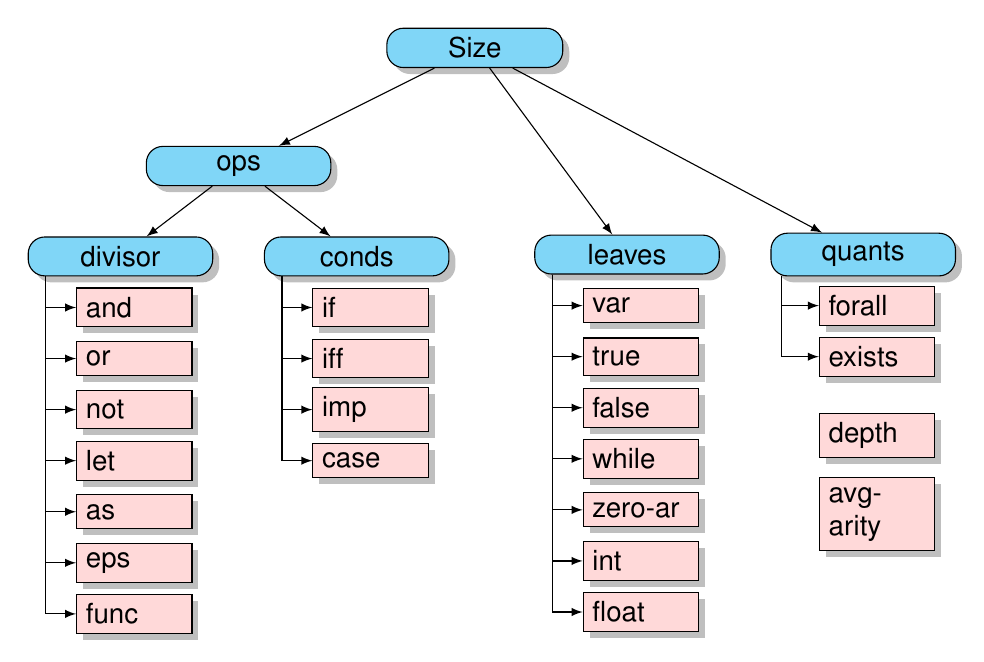
\begin{tikzpicture}[
	level 1/.style={sibling distance=30mm},
	edge from parent/.style={->,draw},
	>=latex]
	
	\node[root]{Size}
	child {node[level 2] (c0) {ops}
		child {node[level 2, yshift=10pt] (c1) {divisor}}
		child {node[level 2, yshift=10pt] (c2) {conds}}
	}
	child {node[level 2, yshift=-32pt, xshift=55pt] (c3) {leaves}}
	child {node[level 2, yshift=-32pt, xshift=55pt] (c4) {quants}}
	;
	
	\begin{scope}[every node/.style={level 3}]
	\node [below of = c1, xshift=5pt, yshift=10pt] (c11) {and};
	\node [below of = c11, yshift=10pt] (c12) {or};
	\node [below of = c12, yshift=10pt] (c13) {not};
	\node [below of = c13, yshift=10pt] (c14) {let};
	\node [below of = c14, yshift=10pt] (c15) {as};
	\node [below of = c15, yshift=10pt] (c16) {eps};
	\node [below of = c16, yshift=10pt] (c17) {func};
	
	
	\node [below of = c2, xshift=5pt, yshift=10pt] (c21) {if};
	\node [below of = c21, yshift=10pt] (c22) {iff};
	\node [below of = c22, yshift=10pt] (c23) {imp};
	\node [below of = c23, yshift=10pt] (c24) {case};
	
	
	\node [below of = c3, xshift=5pt, yshift=10pt] (c31) {var};
	\node [below of = c31, yshift=10pt] (c32) {true};
	\node [below of = c32, yshift=10pt] (c33) {false};
	\node [below of = c33, yshift=10pt] (c34) {while};
	\node [below of = c34, yshift=10pt] (c35) {zero-ar};
	\node [below of = c35, yshift=10pt] (c36) {int};
	\node [below of = c36, yshift=10pt] (c37) {float};
	
	
	\node [below of = c4, xshift=5pt, yshift=10pt] (c41) {forall};
	\node [below of = c41, yshift=10pt] (c42) {exists};
	
	\node [below of = c42](c43) {depth};
	\node [below of = c43](c44) {avg-arity};
	
	\end{scope}
	% lines from each level 1 node to every one of its "children"
	\foreach \value in {1,...,7}
	\draw[->] (c1.195) |- (c1\value.west);
	
	\foreach \value in {1,...,4}
	\draw[->] (c2.195) |- (c2\value.west);
	
	\foreach \value in {1,...,7}
	\draw[->] (c3.195) |- (c3\value.west);
	
	\foreach \value in {1,...,2}
	\draw[->] (c4.195) |- (c4\value.west);
	
	\end{tikzpicture}
	\caption{Tree illustrating the Why syntactic features counted by traversing the AST.}
	\label{fig:types}
\end{figure}


To extract the structural metrics from the logical formul\ae, we traversed the abstract syntax tree (AST) representation. 
We made use of the \why OCaml API to do this. 
Our approach is similar to the method used internally by \why to derive a \textit{shape} string from an interactive proof session \cite{why:preserving}. 
The purpose of shape strings in this context is to track changes in the POs and avoid re-proving files unnecessarily. 
The shape acts as a minimal fingerprint representing the structure of the PO formula. 
Instead of producing a string after traversing the AST, our process simply counts the syntactic features of the formula to construct a feature vector.

Fig. \ref{fig:types} lists the predictor variables that were used in our study.  
All of these are (integer-valued) metrics that can be calculated by analysing the \textsf{Why3} goal statement, and are similar to the \textit{Syntax} metadata category for proof obligations written in the TPTP format \cite{TPTP}. 

The features shown in pink rectangles in Fig. \ref{fig:types} are counted individually by traversing the AST. 
The rounded blue nodes represent metrics that are the sum of their children in the tree. 
The metrics represented by pink rectangles measure syntactic features and are self-explanatory except for the following:
\begin{itemize}
	\item[\textbf{zero-ar}] The number of functions which do not take any arguments (i.e. zero-arity functions)
	\item[\textbf{depth}] The depth of the AST
	\item[\textbf{avg-arity}] The total number of arguments for all functions which are children of the \textit{divisor} node, divided by the value of \textit{divisor}
\end{itemize}   

\textit{Size} measures the size the expression and is the sum of \textit{ops} (the number of operators), \textit{leaves} (the number of leaf nodes in the AST), and \textit{quants} (the number of quantifiers). 

\subsubsection{Example: first\_last lemma}

As a minimal illustrative example, we refer to the code listing in Fig.\ref{fig:code}. 
This code is one of the 13 \textit{Why} proof obligation goals from the \texttt{edit\_distance.mlw} file in the \textit{Why3} examples directory. 
The entire program verifies and algorithm which finds the ``edit distance''\footnote{\url{https://en.wikipedia.org/wiki/Edit_distance}} similarity measure between two strings.  
Informally, this intermediate lemma checks that the same words are produced by (i) prepending a word (minus its first letter \textit{a}) with \textit{a} and (ii) appending a word (minus its last letter \textit{b}) with \textit{b}. 
A representation of the parse tree from this lemma is shown in Fig. \ref{fig:tree}. The reader will note that the zero-arity function \textit{Nil} is a leaf node in the tree, while all other functions (\textit{Cons, =, ++, length}) and operators (\textit{and}) have an arity > 0. 

Table \ref{table:examplemetrics} shows the non-zero metrics used to describe the formula for predictive purposes.

\begin{figure}
	\centering 
	\lstinputlisting[language=ML, firstline=60, lastline=62]{edit_distance.txt}
	\caption{ \textit{WhyML} code for the \textit{first\_last} lemma in \textit{edit\_distance.mlw}}
	\label{fig:code}
\end{figure}

\begin{figure}
	\centering
	\includegraphics[width=\textwidth]{code}
	\caption{The parse tree extracted from the \textit{first\_last} goal (Fig. \ref{fig:code})}
	\label{fig:tree}
\end{figure}

%%

% 	"and": 1.0,
% 	"exists": 1.0,
% 	"n_quants": 2.0,
% 	"zero_ar": 1.0,
% 	"n_branches": 7.0,
% 	"n_ops": 9.0,
% 	"var": 6.0,
% 	"size": 17.0,
% 	"avg_op_arity": 1.55
% 	"forall": 1.0,
% 	"func": 8.0,
% 	"divisor": 9.0,
% 	"depth": 7.0,

%% 

\begin{table}
	\centering
	\caption{Non-zero metrics calculated for \textit{first\_last}} 
	\label{table:examplemetrics}
	\begin{tabular}
		{|r|r|c|r|r|c|r|r|} \hline
		Metric&Value&&Metric&Value&&Metric&Value \\ \hline
		\texttt{and}&1&&\texttt{exists}&1&&\texttt{forall}&1 \\ \hline
		\texttt{var}&6&&\texttt{func}&8&&\texttt{quants}&2 \\ \hline
		\texttt{ops}&9&&\texttt{leaves}&7&&\texttt{depth}&7 \\ \hline
		\texttt{size}&17&&\texttt{divisor}&9&& \texttt{avg\_arity}&1.55 \\ 
		\hline
		\texttt{zero\_ar}&1&& & && & \\ \hline	
	\end{tabular}
\end{table}


\section{Dependent/Response variables}
%Measurement of dynamic properties
\label{sec:dependant}

Our evaluation of the performance of a solver depends on two factors: the time taken to calculate that result, and the solver's output as interpreted by \why.

\subsection{Execution time}
%mention the rationale behind choosing 10 seconds as a reasonable time limit
In order to accurately measure the time each solver takes to return an answer, we used a measurement framework specifically designed for use in competitive environments. 
The BenchExec \cite{ Beyer2016,benchexec} framework was developed by the organisers of the SVCOMP \cite{SVCOMP} software verification competition to reliably measure CPU time, wall-clock time and memory usage of software verification tools. 
We recorded the time spent on CPU by each SMT solver for each proof obligation. 

\subsubsection{Accounting for randomness with confidence intervals}

To account for random errors in measurement introduced at each execution, we used the methodology described by Lilja \cite{LiljaJ} to obtain an approximation of the true mean time. 
A 90\% confidence interval was used with an allowed error of $\pm$3.5\%.   



%By inspecting our data, we saw that most \textit{Valid} and \textit{Invalid} answers returned very quickly, with \textit{Unknown} answers taking slightly longer, and \textit{Failure/Timeout} responses taking longest. We took the relative utility of responses to be $Valid >$ $Invalid>Unknown>Timeout>Failure$ which can be read as ``it is better for a solver to return a \textit{Valid} response than \textit{Timeout}'', etc. A simple function allocates a cost to each solver $S$'s response to each goal $G$:
%\[\small
%cost(S,G) = 
%\begin{cases}
%time_{S,G}, \text{ if answer}_{S,G} \in \lbrace Valid, Invalid \rbrace \\
%time_{S,G} + \text{timeout}, \text{ if answer}_{S,G} = Unknown \\
%dist((time_{S,G},\text{timeout}), (0,0)), \text{if answer}_{S,G} \in \lbrace Timeout, Failure \rbrace
%\end{cases}
%\]
%
%Thus, to penalise the solvers that return an \textit{Unknown} result, the timeout limit is added to the time taken, while solvers returning \textit{Timeout} or \textit{Failure} are further penalised by taking the Euclidean distance from $(0,0)$ to the point defined by the (time taken, timeout limit). This function ensures the best-performing solvers always have the lowest costs. A ranking of solvers for each goal in order of decreasing relevance is obtained by sorting the solvers by ascending cost.
%
%Since our cost model depends on the timeout value chosen, we need to choose a value that does not favour any one solver.  To establish a realistic timeout limit, we find each solver's ``Peter Principle Point'' \cite{Sutcliffe200139}. In resource allocation for theorem proving terms, this point can be defined as the time limit at which more resources will not lead to a significant increase in the number of goals the solver can prove. 

Fig. \ref{fig:line_graph} shows the number of \textit{Valid/Invalid/Unknown} results for each prover when given a timeout value of 60 seconds. 
This value was chosen as an upper limit, since a timeout value of 60 seconds is not realistic for most software verification scenarios.  \textsf{Why3}, for example, has a default timeout value of 5 seconds. 
From Fig. \ref{fig:line_graph} we can see that the vast majority of useful responses are returned very quickly. 

By satisfying ourselves with being able to record 99\% of the useful responses which would be returned after 60 seconds, a more reasonable threshold is obtained for each solver. This threshold ranges from 7.35 secs (veriT) to 9.69 secs (Z3-4.3.2). Thus we chose a value of 10 seconds as a representative, realistic timeout that gives each solver a fair opportunity to return decent results.     

\begin{figure}
	\centering
	\includegraphics[width=\linewidth]{line_graph}
	\caption{The cumulative number of \textit{Valid/Invalid/Unknown} responses for each solver. The plot uses a logarithmic scale on the time axis for increased clarity at the low end of the scale. The chosen timeout limit of 10 secs (\textit{dotted vertical line}) includes 99\% of each solver's useful responses}
	\label{fig:line_graph}
\end{figure}


%Container-based timings using \textit{BenchExec}


\subsection{Prover output}

When a solver is sent a goal by \textsf{Why3}, it returns an answer $A$ where $A$ is one of $\lbrace Valid,Invalid,Unknown,Timeout,Failure \rbrace$. As can be seen from Table \ref{table:avgtimes} and Fig. \ref{fig:barcharts}, not all goals can be proved Valid or Invalid. Such goals usually require the use of an interactive theorem prover to discharge goals that have been inductively defined. Sometimes a splitting transformation needs to be applied to simplify the goals before they are sent to the solver. Our tool does not perform any transformations to goals other than those defined by the solver's \textsf{Why3} driver file. In other cases, more time or memory resources need to be allocated in order to return a conclusive result. We address the issue of resource allocation in the next section.    




\chapter{Choosing a Prediction Model}
\thispagestyle{nohead}
\label{Prediction}

This chapter will evaluate the effectiveness of a number of machine learning algorithms at predicting the most appropriate SMT solver to use on any (unseen) \why~PO.
Our goal in this thesis is to construct a ``meta-solver'' or \textit{portfolio} solver which chooses from a range of tools in order to prove more goals than a single solver is capable of.
We motivate the need for a portfolio solver with an analysis of our dataset 
in Sec. \ref{sec:portfolio-benefit}. 
More details about the type of prediction task chosen for the evaluation of ML algorithms is given in Sec. \ref{sec:reg-class}, with an introduction to a number of theoretical and practical strategies chosen for comparison in Sec. \ref{sec:theoretical} and \ref{sec:practical}. A more detailed introduction to the six prediction models (introduced previously in Sec. \ref{sub:lrsvmmml} and Table \ref{table:algorithms}) is given in Sec. \ref{pred:choosing} before the results of their comparison is discussed. We end this chapter with a more detailed look at the model chosen for use in the actual implementation of \where~.

\section{The benefit of portfolio-solving in \why}
\label{sec:portfolio-benefit}

\newcolumntype{Z}{>{\raggedleft\arraybackslash}X} 
\begin{table}
	\caption[Results of running 8 solvers on the example \why~programs]{Results of running 8 solvers on the example \why~programs.  Also included is a theoretical solver  $ \mathcal{TS}$, which always returns the best answer in the fastest time.}
	\begin{tabularx}{1.1\textwidth}{@{}l|ZZZ|ZZZ|ZZZ@{}}
		\toprule
		{} & \multicolumn{3}{c|}{\textbf{File}} & \multicolumn{3}{c|}{\textbf{Theory}} & \multicolumn{3}{c}{\textbf{Goal}} \\
		{} & \# proved & \% proved & Avg time & \# proved & \% proved & Avg time & \# proved & \% proved & Avg time \\
		\midrule
		$ \mathcal{TS}$ & \textbf{48} & \textbf{37.5\%} & \textbf{1.90} & \textbf{190} & \textbf{63.8\%} & \textbf{1.03} & \textbf{837} & \textbf{79.9\%} & \textbf{0.42} \\
		\textbf{Alt-Ergo-0.95.2} & 25 & 19.5\% & 1.45 & 118 & 39.6\%& 0.77 & 568 & 54.2\% & 0.54 \\ 
		\textbf{Alt-Ergo-1.01} & 34 & 26.6\% & 1.70 & 142 & 47.7\% & 0.79 & 632 & 60.3\% & 0.48 \\ 
		\textbf{CVC3} & 19 & 14.8\% & 1.06 & 128 & 43.0\% & 0.65 & 597 & 57.0\% & 0.49 \\ 
		\textbf{CVC4} & 19  & 14.8\% & 1.09 & 117 & 39.3\% & 0.51 & 612 & 58.4\% & 0.37 \\ 
		\textbf{veriT} & 5 & 4.0\% & 0.12 & 79 & 26.5\% & 0.20 & 333 & 31.8\% & 0.26 \\ 
		\textbf{Yices} & 14 & 10.9\% & 0.53 & 102 & 34.2\% & 0.22 & 368 & 35.1\% & 0.22 \\ 
		\textbf{Z3-4.3.2} & 25 & 19.5\% & 0.56 & 128 & 43.0\% & 0.36 & 588 & 56.1\% & 0.38 \\ 
		\textbf{Z3-4.4.1} & 26 & 20.3\% & 0.58 & 130 & 43.6\% & 0.40 & 581 & 55.4\% & 0.35 \\ 
		\bottomrule
	\end{tabularx}
	\label{table:avgtimes}
\end{table} 


Now that the SMT solvers to be supported by \where~have been identified and an appropriate dataset for training and testing purposes has been chosen, we can make a preliminary and exploratory analysis of the behaviour of the SMT tools on the particular data. 
We aim to make a case for portfolio-solving as an effective method for discharging POs in the \why~system.

We refer the reader to Table \ref{table:avgtimes} which shows the results of running 8 solvers on the example \why~programs with a timeout value of 10 seconds. 
The entire dataset is used in this case. 
WhyML files are modularised as a number of \textit{theories}. The \why~IVL identifies the \textit{goals} which need to be proven in order for the theory (and in turn the entire file) to be verified as correct. 
Our dataset of 128 WhyML files consists of 289 theories, which in turn generate 1048 goals. 
Aside from the number of each modular construct proved by the solver (left sub-column), the percentage this number represents of the total is given (centre sub-column) and the average time taken to prove each construct (as measured using the process described in Sec. \ref{sub:confidence}) is given in the right sub-column. 

Table \ref{table:avgtimes} also shows the results for a \underline{T}heoretical \underline{S}olver $ \mathcal{TS} $. 
$ \mathcal{TS} $ is the best solver, from the eight SMT solvers measured, chosen on a per-goal basis. 
For example, if a file contains one theory which consists of three goals, and the best-performing solver is CVC4 for the first goal, Yices for the second, and CVC3 for the third, the result for $\mathcal{TS}$ on that file is the sum of the results for CVC4 on the first goal, Yices on the second, etc.
We define what is means for a solver to be the \textit{best} in the next subsection.

It is important not to confuse $\mathcal{TS}$ with the theoretical \textsf{Best} ranking introduced in Sec. \ref{sec:strategies}. 
$\mathcal{TS}$ refers to a single solver (and hence is directly comparable to the other eight SMT solvers in Table \ref{table:avgtimes}), while \textsf{Best} refers to a \textit{ranking} which uses all eight solvers\footnote{$\mathcal{TS}$ is, in fact, the result of using the top-ranking solver from \textsf{Best} and stopping.}.


The theoretical solver $\mathcal{TS}$ shows the benefit of being able to use the most appropriate solver for each PO: 205 more goals are provable --- an increase of 19.6\% --- over the best single solver (Alt-Ergo version 1.01). 

\subsection{The relative utility of solver responses}

To make assertions about the relative performance of different solvers on the same goal, a definition of the relative \textit{utility} of solver responses is required.
Should a solver that returns an answer of \textit{Valid} in 5 seconds be seen as ``worse'' than one that returns \textit{Unknown} in 0.5 seconds? 
Likewise, should the solver returning \textit{Failure} after 1 second be penalised more severely than one returning \textit{Timeout} after the maximum time limit?

We define a total ordering for response utility as 
\[
Valid > Invalid > Unknown > Timeout > Failure
\]  
the reasoning being that a \textit{Failure} response usually signals a fatal error in the logic encoding for that solver/goal pair, and the learning algorithm should be discouraged from choosing a failing solver for the particular goal characteristics in question. 
As discussed in Sec. \ref{sub:timeout-limit} of the previous chapter, \textit{Unknown} answers are returned quickly in general, and should not be penalised as much as \textit{Timeout} responses. 
Solvers which reach the timeout limit are unlikely to return a \textit{Valid} or \textit{Invalid} response give more time (illustrated clearly by Fig. \ref{fig:line_graph}).
Solvers returning the same answer are ranked according to runtime --- with faster solvers being preferred.

This method for defining relative performance has similarities to the scoring structure for ATPs competing in SV-COMP \cite{Beyer2016, SVCOMP}, with some important differences. 
Although the notion of ``false positive'' and ``false negative'' responses is not applicable in the SMT domain, a ``true positive'' is scored marginally higher than a ``true negative''. 
In contrast, \textit{Unknown, Timeout} and \textit{Failure} responses are not treated separately by the SV-COMP model --- they all fall under the \textit{Unknown} response category and receive a score of zero.

A further refinement to our scoring model was necessary in order for the prediction models to operate effectively. 
The definition of the \textit{cost} function we applied to solver results is given in Sec. \ref{sub:scoring} of this chapter. 

\section{Classification and regression}
\label{sec:reg-class}

Machine learning prediction tasks can be separated into two categories: those involving the \textit{classification} of a variable into discrete categories or classes, and those predicting a continuous-valued variable directly --- \textit{regression} tasks.
This section will discuss some of the options considered when designing \where's prediction task.

\subsection{Predicting the single best solver} This option involves a multi-class classification task: the classes involved are the eight SMT solvers.
Each PO is classified as belonging in one class. 
This direction was rejected as some benefits associated with portfolio-solving were lost: if the PO is misclassified, the performance of the portfolio solver suffers severely.
\subsection{Predicting the best \textit{ranking} of solvers} Again, this option is a multi-class classification task. 
Instead of predicting a single solver, however, the task involves predicting the entire ranking of eight solvers. 
The benefit of obtaining a ranking is the flexibility it affords in calling SMT solvers sequentially or in parallel.
If the first solver fails or is mispredicted as being the best, the next best predicted solver is called, and so on.
With 8 SMT solvers there are 8! rankings --- far too many to be reasonable for a classification task --- leading to this approach being rejected.
There were no examples of many possible rankings in the training data - making the prediction of such rankings on unseen instances impossible.
\subsection{Predicting solver runtime and response separately}
This approach involves two separate tasks, each predicting a characteristic of the solver's performance. 
One algorithm would attempt to predict the response class (i.e. \textit{Valid, Invalid}, etc.) while another would attempt to predict the solver runtime.
The former task is a multi-class classification task with five classes, while the latter is a regression task.
This method has the advantage of affording the user flexibility in how to choose the ultimate ranking: if fast responses are preferred over \textit{Valid} answers.
This flexibility comes at the price of complexity, however: two accurate predictors, a classifier and regressor, are required instead of one.
\subsection{Combining the prediction of solver response and runtime}
This option uses a cost function to combine the two solver response variables as a single real-valued number which is used for ranking the solvers.
Using this method,  

\subsection{The Cost Function}
\label{sub:scoring}
%maybe leave until it is fixed

\section{Ranking strategies}
\label{sec:strategies}

The following ranking strategies provide a basis by which we can compare 

\subsection{Theoretical \textsf{Best}}
\subsection{Theoretical \textsf{Random}}
\subsection{Theoretical \textsf{Worst}}
\subsection{\textsf{Fixed}}

\section{Choosing the most effective algorithm}
\label{pred:choosing}
\begin{figure}
	\centering
	\includegraphics[width=0.9\linewidth]{Figures/Chapter4}
	\caption{Overview of the process used to derive the \where~prediction model}
	\label{fig:Chapter4}
\end{figure}

\subsection{Train / Test Split}
\subsection{Instance Weighting}
\subsection{Normalised Distributed Cumulative Gain}
\subsection{Mean Average Error}
%\subsection{The prediction of score as a regression task}
%\subsection{The prediction of \textit{result} as a classification task}
%\subsection{The prediction of \textit{time} as a regression task}
%\subsection{The prediction of \textit{time} as a classification task}
%\subsubsection{Binarization}
%\subsubsection{Multiclass via binning}
%\subsection{The prediction of score as an ensemble task}
%\subsection{The prediction of score as a multi-label task} 
\subsection{Properties of multi-output problems}
\label{sub:multi}

\section{The chosen model}
\label{sec:chosen}

 
\chapter{Experimental Results, Evaluation and System Integration}% Main chapter title

\label{Results} % For referencing the chapter elsewhere, use \ref{LitReview} 

%----------------------------------------------------------------------------------------
\section{Introduction to the evaluation metrics}
\subsection{Normalised Distributed Cumulative Gain}
\subsection{Mean Average Error}
\section{Predicting prover result}
\section{Predicting execution time}
\section{Predicting score directly}
\subsection{Predict each score function individually\dots}
\section{System integration}
\subsection{Architecture of a \why{} plugin}
\subsection{Timing the integrated system}
 
\chapter{Evaluating \where~on Test Data}% Main chapter title
\thispagestyle{nohead}
\label{Evaluation} 
%----------------------------------------------------------------------------------------

This chapter will evaluate \where's portfolio algorithm on the held-back test data.
The randomly-selected test set represents 25\% of the entire number of POs and consists of 32 WhyML files, 77 theories and 263 goals  (see Sec. \ref{sub:config}).
In addition to evaluating \where~'s \textit{predictions}, the OCaml implementation (detailed in the previous chapter) will be discussed in terms of its efficiency.   
We perform our evaluation guided by three Evaluation Questions:
\begin{itemize}
	\item[EQ1:] \textbf{How does \where~perform in comparison to the eight SMT solvers?}\\
	The importance of this question is obvious: the success of \where~depends on its improvement over the status quo. In the case of discharging \why~POs, the status quo is represented as the use of a single solver.
	\item[EQ2:] \textbf{How does \where~perform in comparison to the three theoretical strategies?}\\
	The theoretical strategies introduced in Sec. \ref{sec:strategies} provide a fairer basis for comparison than a single solver by taking multiple solver calls per PO into consideration.
	As a reminder for the reader, the \textsf{Best Ranking} always chooses solvers in the order of ascending cost, \textsf{Random Ranking} is the average result of running \textit{every} possible permutation of the eight solvers, and \textsf{Worst Ranking} is the inverse of \textsf{Best Ranking}: it is the ranking of solvers in order of \textit{descending} cost. 
	\item[EQ3:] \textbf{What is the time overhead of using \where~to prove \why~goals?}\\
	The feature extraction and solver scheduling processes incur a time cost. This evaluation criterion measures whether this cost represents a significant proportion of \where~'s overall solving time.    	
\end{itemize}
%The chapter is organised around answering questions raised by each of the three criteria in turn.
This chapter answers each Evaluation Question in turn.
Threats to the validity of our study are discussed in Sec. \ref{sec:threats}. 

\section{EQ1: How does \where~perform in comparison to the eight SMT solvers?}

\label{sec:eq1}

\begin{table}
	\caption[Results for eight solvers, \where~and three strategies on test set]{Number of files, theories and goals proved by each strategy and individual solver. The percentage this represents of the total 32 files, 77 theories, 263 goals, and the average time in seconds, are also shown.}
	\begin{tabularx}{1.1\textwidth}{@{}l|ZZZ|ZZZ|ZZZ@{}}
		\toprule
		{} & \multicolumn{3}{c|}{\textbf{File}} & \multicolumn{3}{c|}{\textbf{Theory}} & \multicolumn{3}{c}{\textbf{Goal}} \\
		{} & \# proved & \% proved & Avg time & \# proved & \% proved & Avg time & \# proved & \% proved & Avg time \\
		\midrule
		\where & 11 & 34.4\% & 1.39 &  44 & 57.1\% & 0.99 & 203 & 77.2\% & 1.98 \\
		\textsf{Best Rank.} & \downbar  & \downbar & 0.25 & \downbar & \downbar & 0.28 & \downbar & \downbar & 0.37 \\
		\textsf{Random Rank.} & \downbar & \downbar & 4.19 & \downbar & \downbar & 4.02 & \downbar & \downbar & 5.70 \\
		\textsf{Worst Rank.} & \upbar & \upbar & 14.71 & \upbar & \upbar & 13.58 & \upbar & \upbar & 18.35 \\
		%\textbf{\textsf{Where4} (tree)} & '' & '' & 4.08 & '' & '' & 2.52 & '' & '' & 3.50 \\
		\midrule
		\textbf{Alt-Ergo-0.95.2} & 8 & 25.0\% & 0.78 & 37 & 48.1\%& 0.26 & 164 & 62.4\% & 0.34 \\ 
		\textbf{Alt-Ergo-1.01} & 10 & 31.3\% & 1.07 & 39 & 50.6\% & 0.26 & 177 & 67.3\% & 0.33 \\ 
		\textbf{CVC3} & 5 & 15.6\% & 0.39 & 36 & 46.8\% & 0.21 & 167 & 63.5\% & 0.38 \\ 
		\textbf{CVC4} & 4  & 12.5\% & 0.56 & 32 & 41.6\% & 0.21 & 147 & 55.9\% & 0.35 \\ 
		\textbf{veriT} & 2 & 6.3\% & 0.12 & 24 & 31.2\% & 0.12 & 100 & 38.0\% & 0.27 \\ 
		\textbf{Yices} & 4 & 12.5\% & 0.32 & 32 & 41.6\% & 0.15 & 113 & 43.0\% & 0.18 \\ 
		\textbf{Z3-4.3.2} & 6 & 18.8\% & 0.46 & 31 & 40.3\% & 0.20 & 145 & 55.1\% & 0.37 \\ 
		\textbf{Z3-4.4.1} & 6 & 18.8\% & 0.56 & 31 & 40.3\% & 0.23 & 145 & 55.1\% & 0.38 \\ 
		\bottomrule
	\end{tabularx}
	\label{table:avgtimes2}
\end{table}

\begin{figure}
	\centering
	\includegraphics[width=\linewidth]{barcharts2}
	\caption[The relative amount of Valid/Unknown/Timeout/Failure answers from the eight SMT solvers, \where, and three theoretical strategies.]{The relative amount of Valid/Unknown/Timeout/Failure answers from the eight SMT solvers, \where~(pre-solver = Alt-Ergo-1.01), and three theoretical strategies on the 263 test POs (with a timeout limit of ten seconds).}
	\label{fig:barchart2}
\end{figure}


When each solver in \textsf{Where4}'s ranking sequence is run on each goal, the maximum amount of files, theories and goals are provable. 
As previously mentioned in Sec. \ref{sub:worst} and as Table \ref{table:avgtimes2} shows, the difference between \where~and the set of reference theoretical strategies (\textsf{Best Ranking}, \textsf{Random Ranking}, and \textsf{Worst Ranking}) is the amount of time taken to return the \textit{Valid/Invalid} result. 
Compared to the eight SMT solvers, the biggest increase is on individual goals: \textsf{Where4} can prove 203 goals, which is 26 (9.9\%) more goals than the next best single SMT solver, Alt-Ergo-1.01.

As is shown by Table \ref{table:avgtimes2}, the average time taken for \textsf{Best Ranking} to return an answer of \textit{Valid} is not necessarily less than that of an individual solver. 
As \textsf{Best Ranking} can return \textit{Valid} for all provable POs -- more than any individual solver --
it is the number of \textit{Valid} answers, rather than any inefficiency, that is responsible for this slightly slower average time.  

The average time \where~takes to prove these goals 
(using Algorithm \ref{algo:where4}) 
is significantly better than the \textsf{Random Ranking} strategy.
It is, however, lagging behind the time recorded by the \textsf{Best Ranking} strategy. 

In comparison to the eight SMT solvers, the average time taken by \where~to prove each of the 203 goals is high. 
This tells us that \where~can perform badly with goals which are not provable by many SMT solvers: expensive \textit{Timeout} results are chosen before the \textit{Valid} result is eventually returned. 
In the worst case, \where~may try all eight solvers in sequence, timing out for each solver, whereas each individual solver does this just once. 
Thus, while having access to more solvers can allow more goals to be proved (if there are goals uniquely-provable by the solvers such as those identified in Table \ref{table:unique}), there is also a time penalty associated with portfolio-based solvers in these circumstances.
This issue has previously been identified by Amadini et al. in their studies on portfolio solvers for constraint programming \cite{Amadini2013} and constraint optimisation \cite{Amadini2016} where portfolio performance was found to degrade as the number of constituent solvers increased.

The multiple timeout issue raises the question of whether it is fair to compare \where~to individual solvers. 
Any ranking strategy will be able to prove the maximum number of files, theories and goals, but unless the best solver is consistently placed high in the ranking, it could take a significantly longer time to do so than even the worst-performing individual solver.   

We remind the reader of the \textsf{Choose Single} solver introduced in Sec. \ref{sec:portfolio-benefit}.
\textsf{Choose Single} is the \textit{best single solver} as chosen on a per-goal basis.
It provided a motivation for the use of portfolio-solving on the \why~platform by proving the maximum number of goals in the shortest amount of time.
We mentioned that \textsf{Choose Single} is equivalent to choosing  the top-ranking solver from \textsf{Best Ranking} and stopping.
We return to this concept in Fig. \ref{fig:barchart2} which is similar to Fig. \ref{fig:barcharts} in that it shows the relative amount of Valid/Unknown/Timeout/Failure answers from the eight SMT solvers. 
Also shown (on the right) are results obtainable by using the top solver (only) with the three ranking strategies (where \textsf{Best Ranking} $\equiv$ \textsf{Choose Single}) and the \where~predicted ranking (after pre-solving with Alt-Ergo version 1.01).


\begin{algorithm}
	\caption{Returning answers and runtimes from \where~solver rankings using a cost threshold: A minor modification to Alg. \ref{algo:where4} with an additional stopping condition in the \textbf{while} loop}
	\KwIn{$P$, a \why~program;\\ 
		$R$, a static ranking of solvers for pre-proving; \\
		$\phi$, a timeout value; \\ 
		$\mu$, the cost threshold}
	\KwOut{$\langle A,T\rangle$ where \\
		$A$ = the best answer from the solvers; \\
		$T$ = the cumulative time taken to return $A$}
	\Begin{
		\tcc{pre-solving}
		$S \leftarrow BestInstalled(R) $ \\				
		$\langle A,T \rangle \leftarrow Call(P, S, 1)$ \\
		\If{$A \in \lbrace Valid, Invalid \rbrace $}
		{\Return{$\langle A,T \rangle$}}
		$F \leftarrow ExtractFeatures(P) $ \\
		$R \leftarrow PredictRanking(F) $ \\
		\tcc{the predicted cost of $S$ is an additional stopping condition}
		\While{$A \notin \lbrace Valid, Invalid \rbrace \wedge R \neq \emptyset \wedge Cost(S) \leq \mu$}
		{$S \leftarrow BestInstalled(R) $ \\	
			$\langle A_S,T_S \rangle \leftarrow Call(P, S, \phi)$ \\
			$T \leftarrow T + T_S$  \\
			\If{$A_S > A$}
			{	
				$A \leftarrow A_S$ }
			\tcc{remove $S$ from the set of solvers $R$}
			$R \leftarrow R \setminus \lbrace S \rbrace$}
		\Return{$\langle A,T\rangle$}}
	\label{algo:threshold}
	
\end{algorithm}

The 62 \text{Valid} answers returned by the top solver from the \textsf{Worst Ranking} (i.e. the worst solver) represent the trivial POs solvable by all eight solvers. 
Likewise, the 60 goals for which \textsf{Best Ranking} did not return a \textit{Valid} or \textit{Invalid} answer could not be proved by any solver.

The results show that limiting the portfolio solver to just using the best predicted individual solver eliminates the multiple time-out overhead yet reduces the number of goals provable by \where.
This number of goals -- 184 -- is still more than the best-performing individual SMT solver, Alt-Ergo version 1.01.  

In an effort to compare \where~to individual SMT solvers, Table \ref{table:avgtimes2} and Fig. \ref{fig:barchart2} show results at two extremes of a spectrum: using all solvers available, and only using one.
In the next subsection we describe a method to calibrate the use of \where~by using the predicted cost of each solver. 


\subsection{Use of a cost threshold}
\label{sub:threshold}

To balance the time-taken-versus-goals-proved trade-off associated with the two approaches above, we introduce the notion of a \textit{cost threshold} as another method of comparing \where~to individual SMT solvers.
\where's use of a cost threshold constitutes a minor adjustment to Alg. \ref{algo:where4} and is detailed in Alg. \ref{algo:threshold}. 
After pre-solving, solvers with a predicted cost above this threshold are not called. 
If every solver's cost is predicted to be above the threshold $\mu$, the pre-solver's result is returned.
%This modification to Algorithm \ref{algo:where4} is shown in Algorithm \ref{algo:threshold}    

We determine the appropriate value for this threshold by first splitting the training data into model training and validation sets.
The model training set used for this step represents 90\% of the total training set (or 706 POs), while the validation set is made up of 79 POs. 
We train the Random Forest predictor (with pre-solving) before simulating the effect of an increasing cost threshold using the validation set.

\begin{figure}
	\centering
	\includegraphics[width=\linewidth]{thresholds1}
	\caption[Determining a cost threshold]{Determining the appropriate value for a cost threshold (using a validation dataset). (\textit{a: top plot}) The average time taken for \where~to return an answer compared to eight SMT solvers. (\textit{b: bottom plot}) The number of Valid/Invalid answers returned by \where~compared to eight SMT solvers.}
	\label{fig:thresholds1}
\end{figure}  


\begin{figure}
	\centering
	\includegraphics[width=\linewidth]{thresholds2}
	\caption[The effect of using a cost threshold]{The effect of using a cost threshold. (\textit{a: top plot}) The average time taken for \where~to return an answer compared to eight SMT solvers. (\textit{b: bottom plot}) The number of Valid/Invalid answers returned by \where~compared to eight SMT solvers.}
	\label{fig:thresholds2}
\end{figure}



Fig. \ref{fig:thresholds1}a and \ref{fig:thresholds1}b show the effect of varying this threshold when solving POs in the test set.
The top plot (\textit{a}) shows a comparison of the average time taken for \textit{any} answer to be returned (not necessarily \textit{Valid / Invalid}).
The amount of time taken by \where~often depends on the number of solvers called.
The number of solvers called depends on the cost threshold given to \where. 
The solid black line of Fig. \ref{fig:thresholds1}a, shows the increase in average time taken by \where~to return a response as the cost threshold increases.
Fig. \ref{fig:thresholds1}b shows the number of \textit{Valid / Invalid} responses returned by each individual SMT solver as compared to \where~with a range of threshold values.
As the corresponding results for each individual solver are unaffected by the threshold parameter, they are represented by horizontal line segments intersecting with the \where~data in Fig. \ref{fig:thresholds1}a.

We note that even when given a threshold value of zero, 46 POs are proven.
The pre-solving routine (in our case, Alt-Ergo-1.01 given a time limit of one second) is responsible for these results (as the solver cost is never used).
As this figure is larger than the number of provable goals for all but three individual solvers, their results are shown as horizontal lines on the left side of the y-axis.
As in Fig. \ref{fig:thresholds1}a, the results for each individual solver are unaffected by the threshold parameter.

By inspecting these results, we find that a threshold value of seven gives good results.
At this threshold, far more \textit{Valid/Invalid} are returned than the best-performing individual solver (Z3-4.4.1) and they are returned in a faster time (on average) than the fastest-returning solver (Yices).

As the dashed red line in Fig. \ref{fig:thresholds2} shows, a threshold value of seven also performs well on the test data.
These results are shown in numerical form in Table \ref{table:threshold}. 
When \where~is given a cost threshold of five, it can prove the same number of POs as the best-performing solver -- Alt-Ergo-1.01. 
By referring to Fig. \ref{fig:thresholds2}a, we see that at the same cost threshold, it takes a shorter time to return a response, on average, than the fastest SMT solver (which is also Alt-Ergo-1.01).
If the cost threshold is increased to seven, significantly more POs can be proven. 
The average time taken to return a response is approximately equal to that of the four slowest individual solvers on the test data: CVC4, veriT, and both versions of Z3. \\
\\
\textbf{EQ1 Answer:} The cost threshold greatly improves \where's performance in comparison to the individual SMT solvers.
The performance penalties associated with portfolio solvers can be mitigated by defining a cut-off point and trusting that solvers with a predicted cost greater than this value do not need to be called.
We found this point to be about seven for the POs in the \textsf{Why3} example dataset.
The value to choose as a threshold may not be obvious in real-world scenarios with unseen results, however. 


\begin{table}
	\caption[The effect of using a cost threshold]{The effect of using a cost threshold. The average time taken for \where~to return an answer compared and the number of Valid/Invalid answers. Same data as Fig. \ref{fig:thresholds2}}
	\begin{tabularx}{0.9\textwidth}{@{}l|Z|Z|Z|Z|Z|Z@{}}

		\textsc{Threshold} & \textbf{0} & \textbf{1} & \textbf{2} & \textbf{3} & \textbf{4} & \textbf{5} \\
		\midrule
		\textbf{Avg. Time} & 0.37 & 0.37 & 0.48 & 0.53 & 0.98 & 1.77  \\
		\textbf{Num. Proved} & 168 & 168 & 168 & 169 & 173 & 177  \\
		\midrule
		\midrule
		\textsc{Threshold}  & \textbf{6} & \textbf{7} & \textbf{8} & \textbf{9} & \textbf{10} & \textbf{11}  \\
		\midrule
		\textbf{Avg. Time} & 2.72 & 4.59 & 6.55 & 8.74 & 10.31 & 11.89  \\
		\textbf{Num. Proved} & 183 & 192 & 192 & 195 & 197 & 199 \\
		\midrule
		\midrule
		\textsc{Threshold} & \textbf{12} & \textbf{13} & \textbf{14} & \textbf{15} & \textbf{16} & \textbf{17} \\
		\midrule
		\textbf{Avg. Time} & 14.16 & 15.24 & 16.06 & 16.35 & 16.35 & 16.35 \\
		\textbf{Num. Proved}  & 202 & 203 & 203 & 203 & 203 & 203 \\
		
	\end{tabularx}
	\label{table:threshold}
\end{table}

\section{EQ2: How does \where~perform in comparison to the three theoretical strategies?}


\begin{figure}
	\centering
	\includegraphics[width=1.0\linewidth]{line_graph_eval_provers}
	\caption{The time taken by each theoretical strategy and \where~to return all \textit{Valid/Invalid} answers in the test dataset of 263 goals}
	\label{fig:line_graph_eval_provers}
\end{figure}

Fig. \ref{fig:line_graph_eval_provers} compares the time taken for \where~and the three ranking strategies to return \textit{Valid} answers for the 263 POs in the test set.
This experiment is equivalent to running each strategy on all 263 POs in parallel and measuring the time taken for each strategy to return a total of 203 \textit{Valid} answers.
As described in Sec. \ref{sec:strategies}, \textsf{Best Ranking} and \textsf{Worst Ranking} use Alg. \ref{algo:rank} to return their time taken.
\textsf{Random Ranking}'s time measurement is based on the average of 40,320 (i.e. eight factorial, the number of individual rankings) uses of Alg. \ref{algo:rank}.
\where's times are derived from the use of Alg. \ref{algo:where4} with a pre-solver of Alt-Ergo-1.01. 
Although both \where~and \textsf{Random Ranking} finish at approximately the same time, \where~is significantly faster for returning \textit{Valid/Invalid} answers. 
\where's solid line is more closely correlated to \textsf{Best Ranking}'s rate of success than the erratic rate of the \textsf{Random Ranking} strategy. 
Again, we find that \where~struggles to prove a small number of POs.
\textsf{Best Ranking}'s excellent time result shows the capability of a perfect-scoring learning strategy. \\
\\
\textbf{EQ2 Answer:} At almost any point in time from zero seconds to 42.65 seconds, the number of \textit{Valid/Invalid} answers returned by \where~is greater than the number returned by \textsf{Random Ranking}.
This shows that our prediction model is a better choice than selecting a sequence of SMT solvers at random, without any regard to program features or solver capability.
\where's performance on all but the hardest POs is encouraging.
Although \where~cannot compete with \textsf{Best Ranking} yet, the performance of this theoretical strategy is motivation to further improve \where~in the future.   



\section{EQ3: What is the time overhead of using \where~to prove \why~goals?}

\label{sec:eq3}

The timings for \where~in all plots and tables in this chapter are based solely on the performance of the constituent solvers (the measurement of which is discussed in Sec. \ref{sec:dependant}). They do not measure the time it takes for the OCaml binary to extract the static metrics, traverse the decision trees and predict the ranking. 
We have found that this adds (on average) 0.46 seconds to the time \where~takes to return a result for each of the files in the test set. 
On a per goal basis, this is equivalent to an increase in 0.056 seconds.
This overhead is only applied to goals for which pre-solving is unsuccessful.  
For the test set, pre-solving eliminated this overhead for 168 out of 263 POs (see Table \ref{table:threshold}: \where's number of \textit{Valid/Invalid} responses when the cost threshold is zero).

The imitation of an orthodox solver to interact with \why~is more costly: this is due to \why~printing each goal as a temporary file to be read in by the solver individually (see Sec. \ref{sec:why3-integration}). 
As \where~uses the abstract, internal representation of the program, the printing of each goal to the Why format is unnecessary.
The \why~driver mechanism makes this step unavoidable for any supported solver including, of course, the \where~``imitation solver''.

Another issue with calling \where~through \why~is that of applying \why's timeout value to a sequence of solver calls. 
For example, if a user gives \why~a timeout of five seconds for \where~to prove a PO and the first solver called by \where~goes over that limit, the potentially useful answer returned by the second solver in the sequence would not be returned to the user. \\
\\
\textbf{EQ3 Answer:}
While pre-solving is an important heuristic for avoiding the overhead of feature extraction and rank prediction, these processes must be optimised for \where~to be practical as a portfolio solver called from \why.   
Future work will look at a portfolio-solving \why~plugin similar to \where. Tighter integration with the \why~system can be expected to improve the efficiency of such a tool.      
In its current form, \where~is more suited to an initial proving step performed using the stand-alone command line tool.

\section{Threats to Validity}
\label{sec:threats}

In this section we discuss the threats to the validity of the evaluation presented in this chapter.
We categorise threats as either \textit{internal} or \textit{external}.
Internal threats refer to influences that can affect the response variable without the researcher's knowledge and threaten the conclusions reached about the \textit{cause} of the experimental results \cite{experimentation}. 
Threats to external validity are conditions that limit the generalisability and reproducibility of an experiment. 

\subsection{Internal}

The main threat to our work's internal validity is selection bias. All of our training and test samples are taken from the same source. 
We took care to split the data for training and testing purposes on a \textit{per file} basis, as we discussed in Sec. \ref{sub:config}. 
This ensured that \where~was not trained on a goal belonging to the same theory or file as any goal used for testing.
 
The results of running the solvers on our dataset are imbalanced. There were far more \textit{Valid} responses than any other response. 
No goal in our dataset returned an answer of \textit{Invalid} on any of the eight solvers. 
This is a serious problem as \where~would not be able to recognize such a goal in real-world use. 

Use of an independent dataset is likely to influence the performance of the solvers. 
Alt-Ergo was designed for use with the \why~platform -- its input language is a previous version of the Why logic language. 
It is natural that the developers of the \why~examples would write programs which Alt-Ergo in particular would be able to prove. 
Due to the syntactic similarities in input format and logical similarities such as support for type polymorphism, it is likely that Alt-Ergo would perform well with any \why~dataset. We would hope, however, that the gulf between it and other solvers would narrow.

There may be confounding effects in a solver's results that are not related to the independent variables we used (Sec. \ref{sec:independant}). 
We were limited in the tools available to extract features from the domain-specific Why logic language (in contrast to related work on model checkers which use the general-purpose C language \cite{DPVZ15:CAV, MUX} -- as previously discussed in Sec. \ref{sub:lrsvmmml}). 
We made the decision to keep the choice of independent variables simple in order to increase generalisability to other formalisms such as Microsoft's Boogie \cite{Boogie} intermediate language.  

\subsection{External}


The generalisability of our results is limited by the fact that all dependent variables were measured on a single machine.
All data collection was conducted on a single 64-bit machine running Ubuntu 14.04 with a dual-core Intel i5-4250U CPU and 16GB of RAM. 
We believe that the number of each response for each solver would not vary dramatically on a different machine of similar specifications. 
By inspecting the results when each solver was given a timeout of 60 seconds (Fig. \ref{fig:line_graph}), the rate of increase for \textit{Valid/Invalid} results was much lower than that of \textit{Unknown/Failure} results. 
The former set of results are more important when computing the cost value for each solver-goal pair.

Timings of individual goals are likely to vary widely (even across independent executions on the same machine).
% Locally, we used a statistically-accurate mean timing based on a 90\% confidence interval (see Sec. \ref{sec:dependant}). 
It is our assumption that although the actual timed values would be quite different on any other machine, the \textit{ranking} of their timings would stay relatively stable.

A ``typical'' software development scenario might involve a user verifying a single file with a small number of resultant goals: certainly much smaller than the size of our test set (263 goals). In such a setting, the productivity gains associated with using \where~would be minor. 
\where~is more suited therefore to large-scale software verification.


\section{Discussion}
\label{sec:eval-discuss}

By considering the answers to our three Evaluation Questions, we can make assertions about the success of  \where.
The answer to \textbf{EC1}, \where's performance in comparison to individual SMT solvers, is positive.
A small improvement in \textit{Valid/Invalid} responses results from using only the top-ranked solver, while a much bigger increase can be seen by making the full ranking of solvers available for use.
The time penalty associated with calling a number of solvers on an un-provable PO is mitigated by the use of a \textit{cost threshold}.
Judicious use of this threshold value can balance the time-taken-versus-goals-proved trade-off: in our test set of 263 POs, using a threshold value of seven results in 192 \textit{Valid} responses -- an increase of fifteen over the single best solver -- in a reasonable average time per PO (both \textit{Valid} and otherwise) of 4.59 seconds.

There is also cause for optimism in \where's performance as compared to the three theoretical ranking strategies -- the subject of Evaluation Question 2. 
All but the most stubborn of \textit{Valid} answers are returned in a time far better than \textsf{Random Ranking}.
We take this random strategy as representing the behaviour of the non-expert \why~user who does not have a preference amongst the variety of supported SMT solvers.
For this user, \where~could be a valuable tool in the efficient initial verification of POs through the \why~system.    

In terms of time overhead -- the concern of EQ3 -- our results are less favourable, particularly when \where~is used as an integrated part of the \why~toolchain.
The costly printing and parsing of POs slows \where~beyond the time overhead associated with feature extraction and prediction.
At present, due to the diversity of languages and input formats in use for SV (see Sec. \ref{sec:lrsv}), this is an unavoidable pre-processing step enforced by \why~(and is indeed one of the \why~system's major advantages).

Overall, we believe that the results for two out of three Evaluation Questions are encouraging and suggest a number of directions for future work to improve \where.
 

 


\chapter{Threats to Validity}
\section{Construct}
\section{Internal}
\section{External}
\section{Conclusion}

%----------------------------------------------------------------------------------------
%	THESIS CONTENT - APPENDICES
%----------------------------------------------------------------------------------------

\appendix % Cue to tell LaTeX that the following "chapters" are Appendices

% Include the appendices of the thesis as separate files from the Appendices folder
% Uncomment the lines as you write the Appendices

% Appendix A
\chapter{Ocaml Interfaces} % Main appendix title
\thispagestyle{nohead}
\label{App:interfaces} % For referencing this appendix elsewhere, use \ref{AppendixA}

\section*{\texttt{treetypes.mli}}

\lstinputlisting[language={[Objective]Caml}]{/home/andrew/Documents/where4/treetypes.mli}

\section*{\texttt{tree.mli}}

\lstinputlisting[language={[Objective]Caml}]{/home/andrew/Documents/where4/tree.mli}

\pagebreak


\section*{\texttt{mytermcode.mli}}

\lstinputlisting[language={[Objective]Caml}]{/home/andrew/Documents/where4/mytermcode.mli}

\section*{\texttt{get\_predictions.mli}}

\lstinputlisting[language={[Objective]Caml}]{/home/andrew/Documents/where4/get_predictions.mli}

\pagebreak

\section*{\texttt{make\_session.mli}}

\lstinputlisting[language={[Objective]Caml}]{/home/andrew/Documents/where4/make_session.mli}

\chapter{\where~command-line options} % Main appendix title
\thispagestyle{nohead}
\label{App:command} % For referencing this appendix elsewhere, use \ref{AppendixA}

The \textsf{Where4} command-line tool has the following functionality:
\begin{enumerate}
	\item Read in the WhyML/Why file and extract feature vectors from its goals.% formulae.
	\item Find the predicted costs for each of the 8 provers by traversing the random forest, using each goal's feature vector.
	\item Sort the costs to produce a ranking of the SMT solvers.
	\item Use the \textsf{Why3} API to call each solver (if it is installed) in rank order.
	%\item Print the result.
	\item Repeat 4 as necessary until a \textit{Valid/Invalid} response is recorded or all installed solvers have been called.
\end{enumerate}
\chapter{\where~installation options}
\thispagestyle{nohead}
\label{App:install}


As a random forest is just an array of trees, a JSON file containing a single \textit{tree} may be provided instead, if it is specified as such during installation.

%----------------------------------------------------------------------------------------
%	BIBLIOGRAPHY
%----------------------------------------------------------------------------------------

\printbibliography[heading=bibintoc]

%----------------------------------------------------------------------------------------

\end{document}  
